\documentclass[11pt]{article}
\PassOptionsToPackage{dvipsnames}{xcolor}
\usepackage{amsmath, amssymb, amscd, amsthm, amsfonts}
\usepackage{tikz}
\usetikzlibrary{math}
\usetikzlibrary{positioning}
\usepackage{comment}
\usepackage{circuitikz}
\usepackage{graphicx}
\usepackage{hyperref}
\usepackage{amssymb}
\usepackage[makeroom]{cancel}
\oddsidemargin 0pt
\evensidemargin 0pt
\marginparwidth 40pt
\marginparsep 10pt
\topmargin -20pt
\headsep 10pt
\textheight 8.7in
\textwidth 6.65in
\linespread{1.2}

\title{Balanced Mixer Math}
%\author{Sebastian Jorquera}
\date{}

\newtheorem{theorem}{Theorem}
\newtheorem{lemma}[theorem]{Lemma}
\newtheorem{conjecture}[theorem]{Conjecture}

\newcommand{\rr}{\mathbb{R}}

\newcommand{\al}{\alpha}
\DeclareMathOperator{\conv}{conv}
\DeclareMathOperator{\aff}{aff}

\begin{document}

\maketitle

\begin{abstract}

\end{abstract}

\section{Ideal Balanced Mixer}\label{section-introduction}

\begin{figure}[t]
    \centering
    \begin{circuitikz}[scale=0.8, transform shape]
    \draw (0,0) node[coupler, label={[yshift=-1.5cm]RF Hybrid}] (c) {}
    (c.port1) to[short,-o] ++(-2,0)
    (c.port4) to[short,-o] ++(-2,0)
    (c.port4) node[above, left=2cm] {$V_{LO}$}
    (c.port1) node[below, left=2cm] {$V_{RF}$}
    (c.port3) to [diode, l=$V_{D1}$] ++(3,0) to ++(0,-0.45) to[short, -o, label={$out$}] ++(1,0)
    (c.port2) to [diode, invert, l_=$V_{D2}$] ++(3,0) to ++(0,0.45) 
    ;
    \node[above left = 0.9cm and 0.1cm of c.port1] (1) {\scriptsize{$1$}};
    \node[above left = -0.9cm and 0.1cm of c.port4] (4) {\scriptsize{$4$}};
    \node[above right = 0.9cm and 0.1cm of c.port2] (2) {\scriptsize{$2$}};\node[above right = -0.9cm and 0.1cm of c.port3] (3) {\scriptsize{$3$}};
    

\end{circuitikz}
    \caption{Balanced mixer architecture}
    \label{fig:bm_ideal}
\end{figure}


The figure \ref{fig:bm_ideal} shows the typical balanced mixer setup. In our math we are going to use a 90° hybrid with the S matrix of the equation \ref{eq:s_hybrid}.

\begin{equation}
    \label{eq:s_hybrid}
    S = \frac{-1}{\sqrt{2}}
    \begin{pmatrix}
        0 & j & 1 & 0 \\
        j & 0 & 0 & 1 \\
        1 & 0 & 0 & j \\
        0 & 1 & j & 0 
    \end{pmatrix}
\end{equation}



The voltage at the inputs of the hybrid are given \ref{eq:v_lo} where $\eta$ represent the noise of the local oscillator, and the equation \ref{eq:v_rf} is the input of the RF, where $\nu_{usb}=\omega_{lo}+\omega_{lsb}$ and $\nu_{lsb}=\omega_{lo}-\omega_{lsb}$ where $\omega_{usb}$ and $\omega_{lsb}$ will be our IF signals.

\begin{equation}
    \label{eq:v_lo}
    \begin{gathered}
    V_{lo} = \textcolor{red}{V_{lo}\cos(\omega_{lo}t)}+
    \textcolor{Magenta}{\eta_{usb}\cos((\omega_{lo}+\Delta)t+\phi_{usb})} +
    \textcolor{blue}{\eta_{lsb}\cos((\omega_{lo}-\Delta)t+\phi_{lsb})}
    \end{gathered}
\end{equation}

\begin{equation}
    \label{eq:v_rf}
    V_{RF} = \textcolor{ForestGreen}{V_{usb}\cos(\nu_{usb}t)}+\textcolor{orange}{{V_{lsb}}\cos(\nu_{lsb}t)}
\end{equation}


The voltage at the diode 1 should be given by the equation \ref{equation:diode1_general} where for an ideal hybrid $|S_{21}|=|S_{42}|=1$ and $\theta_{42}=\theta_{12}=0$. 
\begin{equation}
    \label{equation:diode1_general}
    V_{D1} = |S_{42}(\omega)|V_{RF} \angle{(-90+\theta_{42}(\omega))} + |S_{21}|V_{lo}\angle{(-180+\theta_{21}(\omega))}
\end{equation}


\begin{equation}
    \begin{gathered}
    V_{D1} = \textcolor{ForestGreen}{|S_{24}(\nu_{usb})| V_{usb}\sin(\nu_{usb}t+\theta_{24}(\nu_{usb}))} + 
    \textcolor{orange}{|S_{24}(\nu_{lsb})|V_{lsb}\sin(\nu_{lsb}t+\theta_{24}(\nu_{lsb}))} \\
    \textcolor{red}{-|S_{21}(\omega_{lo})|V_{lo}\cos(\omega_{lo}t+\theta_{21}(\omega_{lo}))} \\
    \textcolor{Magenta}{-|S_{21}(\omega_{lo}+\Delta)|\eta_{usb}\cos((\omega_{lo}+\Delta)t+\phi_{usb}+\theta_{21}(\omega_{lo}+\Delta))} \\
    \textcolor{blue}{
    -|S_{21}(\omega_{lo}-\Delta)|\eta_{lsb}\cos((\omega_{lo}-\Delta)t+\phi_{lsb}+\theta_{21}(\omega_{lo}-\Delta))
    }
    \end{gathered}
\end{equation}


In the same way we obtain the equation for the voltage in the diode 2
\begin{equation}
    V_{D2} = |S_{34}(\omega)|V_{rf}\angle{(-180+\theta_{34})}+|S_{31}(\omega)|V_{lo}\angle{(-90+\theta_{31}(\omega))}
\end{equation}

\begin{equation}
    \begin{gathered}
        V_{D2} = \textcolor{ForestGreen}{-|S_{34}(\nu_{usb})|V_{usb}\cos(\nu_{usb}t+\theta_{34}(\nu_{usb}))
        }
        \textcolor{orange}{
        -|S_{34}(\nu_{lsb})|V_{lsb}\cos(\nu_{lsb}t+\theta_{34}(\nu_{lsb}))
        }\\
        \textcolor{red}{+|S_{31}(\omega_{lo})|V_{lo}\sin(\omega_{lo}t+\theta_{31}(\omega_{lo}))}\\
        \textcolor{magenta}{+|S_{31}(\omega_{lo}+\Delta)|\eta_{usb}\sin((\omega_{lo}+\Delta)t+\phi_{usb}+\theta_{31}(\omega_{usb}+\Delta))}\\
        \textcolor{blue}{+|S_{31}(\omega_{lo}-\Delta)|\eta_{lsb}\sin((\omega_{lo}-\Delta)t+\phi_{lsb}+\theta_{31}(\omega_{usb}-\Delta))}
    \end{gathered}
\end{equation}

\vspace{1cm}


The typical linearized model of a diode is given by the equation \ref{eq:diode_eq}, to not go crazy with the terms we only look at the second order terms.  We also argue that only the terms that contain $V_{lo}$ are be important for our analysis due the LO is the strongest signal, so the cross terms that does not contain it are neglectable. 

\begin{gather}
    \label{eq:diode_eq}
    I_{D1} = \alpha_0 + \alpha_1 V_{D1} + \alpha_2 \frac{V_{D1}^2}{2}+\ldots \\
    \label{eq:i_d2_0}
    I_{D2} = \beta_1 - \beta_2 V_{D2} + \beta_2 \frac{V_{D2}^2}{2}+ \ldots
\end{gather}

\vspace{2cm}

\begin{equation}
    \label{eq:d1_signal}
    \begin{gathered}
        I_{D1, signal} = \alpha_{2} \biggl[ \textcolor{red}{V_{lo}|S_{21}(\omega_{lo})|}
        \textcolor{ForestGreen}{|S_{24}(\nu_{usb})|V_{usb}}\sin(\textcolor{ForestGreen}{\omega_{usb}t+\theta_{24}(\nu_{usb})}\textcolor{red}{-\theta_{21}(\omega_{lo})})+ \\
        \textcolor{red}{V_{lo}|S_{21}(\omega_{lo})|}
        \textcolor{orange}{|S_{24}(\nu_{lsb})|V_{lsb}}\sin({\textcolor{ForestGreen}{-\omega_{lsb}t+\theta_{24}(\nu_{usb})}-\textcolor{red}{\theta_{21}(\omega_{lo})}})
        \biggr]
    \end{gathered}
\end{equation}

\begin{equation}
    \label{eq:d1_noise}
    \boxed{
    \begin{gathered}
        I_{D1, noise} = \alpha_{2} \biggl[ 
        \textcolor{red}{V_{lo}|S_{21}(\omega_{lo})|}
        \textcolor{Magenta}{(-|S_{21}(\omega_{lo}+\Delta)|\eta_{usb})}\cos(
        \textcolor{Magenta}{\Delta t+\phi_{usb}+\theta_{21}(\omega_{lo}+\Delta)}
        -\textcolor{red}{\theta_{21}(\omega_{lo})}
        ) \\
        +
        \textcolor{red}{V_{lo}|S_{21}(\omega_{lo})|}
        \textcolor{blue}{(-|S_{21}(\omega_{lo}-\Delta)|\eta_{lsb})}\cos(
        \textcolor{blue}{-\Delta t+\phi_{lsb}+\theta_{21}(\omega_{lo}-\Delta)}
        \textcolor{red}{-\theta_{21}(\omega_{lo})}
        )
        \biggr]
    \end{gathered}
    }
\end{equation}

%this is a preliminar result
%\begin{equation}
%    \begin{gathered}
%        I_{D2, signal} = \beta_{2}\biggl[
%            \textcolor{red}{|S_{31}(\omega_{lo})|V_{lo}}
%            \textcolor{ForestGreen}{\bigr(-|S_{34}(\nu_{usb})|V_{usb}\bigl)}
%            \bigl(-\sin(
%            \textcolor{ForestGreen}{\omega_{usb}t+\theta_{34}(\nu_{usb})}
%            \textcolor{red}{-\theta_{31}(\omega_{lo})}) \bigr)+\\
%            \textcolor{red}{|S_{31}(\omega_{lo})|V_{lo}}
%            \textcolor{orange}{\bigr(-|S_{34}(\nu_{lsb})|V_{lsb}\bigl)}
%            \bigl(-\sin(
%            \textcolor{orange}{-\omega_{lsb}t+\theta_{34}(\nu_{lsb})}
%            \textcolor{red}{-\theta_{31}(\omega_{lo})}) \bigr)
%        \biggr]\\ 
%    \end{gathered}
%\end{equation}

\begin{equation}
    \label{eq:d2_signal}
    \begin{gathered}
        I_{D2,signal} = \beta_{2} \biggl[
            \textcolor{red}{|S_{31}(\omega_{lo})|V_{lo}}
            \textcolor{ForestGreen}{|S_{34}(\nu_{usb})|V_{usb}}
            \sin(
            \textcolor{ForestGreen}{\omega_{usb}t+\theta_{34}(\nu_{usb})}
            \textcolor{red}{-\theta_{31}(\omega_{lo})})+\\
            \textcolor{red}{|S_{31}(\omega_{lo})|V_{lo}}
            \textcolor{orange}{|S_{34}(\nu_{lsb})|V_{lsb}}
            \sin(
            \textcolor{orange}{-\omega_{lsb}t+\theta_{34}(\nu_{lsb})}
            \textcolor{red}{-\theta_{31}(\omega_{lo})})
        \biggr]
    \end{gathered}
\end{equation}


\begin{equation}
    \label{eq:d2_noise}
    \boxed{
    \begin{gathered}
        I_{D2,noise} = \beta_{2} \biggl[
        \textcolor{red}{|S_{31}(\omega_{lo})|V_{lo}}
        \textcolor{Magenta}{|S_{31}(\omega_{lo}+\Delta)|\eta_{usb}}
        \cos(\textcolor{Magenta}{\Delta t+\phi_{usb}+\theta_{31}(\omega_{lo}+\Delta)}
        \textcolor{red}{-\theta_{31}(\omega_{lo})}) +\\
        \textcolor{red}{|S_{31}(\omega_{lo})|V_{lo}}
        \textcolor{blue}{|S_{31}(\omega_{lo}-\Delta)|\eta_{lsb}}
        \cos(\textcolor{blue}{-\Delta t+\phi_{lsb}+\theta_{31}(\omega_{lo}-\Delta)}
        \textcolor{red}{-\theta_{31}(\omega_{lo})})
        \biggr]
    \end{gathered}      
    }
\end{equation}


\subsection{Symmetry relations}
Due symmetry we have some equivalence relations, we use $S_{21} = S_{34}$ and $S_{31}=S_{24}$.
Replacing that in the equations \ref{eq:d1_noise} and \ref{eq:d2_noise} we obtain 

\begin{equation}
    \label{eq:d1_noise_sym}
    \boxed{
    \begin{gathered}
        I_{D1, noise} = \alpha_{2} \biggl[ 
        \textcolor{red}{V_{lo}|S_{21}(\omega_{lo})|}
        \textcolor{Magenta}{(-|S_{21}(\omega_{lo}+\Delta)|\eta_{usb})}\cos(
        \textcolor{Magenta}{\Delta t+\phi_{usb}+\theta_{21}(\omega_{lo}+\Delta)}
        -\textcolor{red}{\theta_{21}(\omega_{lo})}
        ) \\
        +
        \textcolor{red}{V_{lo}|S_{21}(\omega_{lo})|}
        \textcolor{blue}{(-|S_{21}(\omega_{lo}-\Delta)|\eta_{lsb})}\cos(
        \textcolor{blue}{-\Delta t+\phi_{lsb}+\theta_{21}(\omega_{lo}-\Delta)}
        \textcolor{red}{-\theta_{21}(\omega_{lo})}
        )
        \biggr]
    \end{gathered}
    }
\end{equation}




\begin{equation}
    \label{eq:d2_noise_sym}
    \boxed{
    \begin{gathered}
        I_{D2,noise} = \beta_{2} \biggl[
        \textcolor{red}{|S_{31}(\omega_{lo})|V_{lo}}
        \textcolor{Magenta}{|S_{31}(\omega_{lo}+\Delta)|\eta_{usb}}
        \cos(\textcolor{Magenta}{\Delta t+\phi_{usb}+\theta_{31}(\omega_{lo}+\Delta)}
        \textcolor{red}{-\theta_{31}(\omega_{lo})}) +\\
        \textcolor{red}{|S_{31}(\omega_{lo})|V_{lo}}
        \textcolor{blue}{|S_{31}(\omega_{lo}-\Delta)|\eta_{lsb}}
        \cos(\textcolor{blue}{-\Delta t+\phi_{lsb}+\theta_{31}(\omega_{lo}-\Delta)}
        \textcolor{red}{-\theta_{31}(\omega_{lo})})
        \biggr]
    \end{gathered}      
    }
\end{equation}


\section{Ideal balanced mixer}

In the ideal world $|S_{ij}| = 1$, $\theta_{i,j}=0$ and $\alpha = \beta$. In this configuration we have that the equation \ref{eq:d1_noise} is the inverse of the equation \ref{eq:d2_noise} and the equation \ref{eq:d1_signal} is equal to \ref{eq:d2_signal}.

In this case the combiner doubles the downconverted RF signal and the removes the noise coming from the LO.


\section{Non ideal balanced mixer}

Looking at the expression of the equations \label{eq:d1_signal}, \label{eq:d1_noise}, \label{eq:d2_signal} and \label{eq:d2_noise} we have two signals that falls in the same frequency component coming from the LSB and the USB. 
In order to study the effect over one frequency component we are going to take $\omega_{lo}+\Delta = \nu_{usb}$ and $\omega_{lo}-\Delta = \nu_{lsb}$ meaning that $\Delta=\omega_{lsb}=\omega_{usb}$. The equations are then:

\begin{equation}
    \label{eq:d1_signal}
    \begin{gathered}
        I_{D1, signal} = \alpha_{2}\textcolor{red}{V_{lo}|S_{21}(\omega_{lo})|}\biggl[ 
        \textcolor{ForestGreen}{|S_{24}(\nu_{usb})|V_{usb}}\sin(\textcolor{ForestGreen}{\Delta t+\theta_{24}(\nu_{usb})}\textcolor{red}{-\theta_{21}(\omega_{lo})}) \\
        -\textcolor{orange}{|S_{24}(\nu_{lsb})|V_{lsb}}\sin({\textcolor{orange}{\Delta t-\theta_{24}(\nu_{lsb})}+\textcolor{red}{\theta_{21}(\omega_{lo})}})
        \biggr]
    \end{gathered}
\end{equation}


\begin{equation}
    \label{eq:d2_signal}
    \begin{gathered}
        I_{D2,signal} = \beta_{2} \textcolor{red}{V_{lo}|S_{31}(\omega_{lo})|} \biggl[
            \textcolor{ForestGreen}{|S_{34}(\nu_{usb})|V_{usb}}
            \sin(
            \textcolor{ForestGreen}{\Delta t+\theta_{34}(\nu_{usb})}
            \textcolor{red}{-\theta_{31}(\omega_{lo})})\\
            -\textcolor{orange}{|S_{34}(\nu_{lsb})|V_{lsb}}
            \sin(
            \textcolor{orange}{\Delta t-\theta_{34}(\nu_{lsb})}
            \textcolor{red}{+\theta_{31}(\omega_{lo})})
        \biggr]
    \end{gathered}
\end{equation}


\begin{equation}
    \label{eq:d1_noise_2}
    \boxed{
    \begin{gathered}
        I_{D1, noise} = -\alpha_{2}\textcolor{red}{V_{lo}|S_{21}(\omega_{lo})|} \biggl[ 
        \textcolor{Magenta}{|S_{21}(\nu_{usb})|\eta_{usb}}\cos(
        \textcolor{Magenta}{\Delta t+\phi_{usb}+\theta_{21}(\nu_{usb})}
        \textcolor{red}{-\theta_{21}(\omega_{lo})}
        )+ \\
        \textcolor{blue}{|S_{21}(\nu_{lsb})|\eta_{lsb}}\cos(
        \textcolor{blue}{\Delta t-\phi_{lsb}-\theta_{21}(\nu_{lsb})}
        \textcolor{red}{+\theta_{21}(\omega_{lo})}
        )
        \biggr]
    \end{gathered}
    }
\end{equation}

\begin{equation}
    \label{eq:d2_noise}
    \boxed{
    \begin{gathered}
        I_{D2,noise} = \beta_{2}\textcolor{red}{V_{lo}|S_{31}(\omega_{lo})|} \biggl[
        \textcolor{Magenta}{|S_{31}(\nu_{usb})|\eta_{usb}}
        \cos(\textcolor{Magenta}{\Delta t+\phi_{usb}+\theta_{31}(\nu_{usb})}
        \textcolor{red}{-\theta_{31}(\omega_{lo})})+\\
        \textcolor{blue}{|S_{31}(\nu_{lsb})|\eta_{lsb}}
        \cos(\textcolor{blue}{\Delta t-\phi_{lsb}-\theta_{31}(\nu_{lsb})}
        \textcolor{red}{+\theta_{31}(\omega_{lo})})
        \biggr]
    \end{gathered}      
    }
\end{equation}

Emulating a FX correlator we will take a Fourier transform over the previous expressions.

\begin{equation}
    \label{eq:d1_signal_fft}
    \begin{gathered}
        I_{D1, signal} = -i\pi\biggl(\delta(\omega-\Delta)-\delta(\omega+\Delta)\biggr)
        \alpha_{2}\textcolor{red}{V_{lo}|S_{21}(\omega_{lo})|}
        \biggl[ \\ 
        \textcolor{ForestGreen}{|S_{24}(\nu_{usb})|V_{usb}}
        e^{i(\textcolor{ForestGreen}{
        \theta_{24}(\nu_{usb})\textcolor{red}{-\theta_{21}(\omega_{lo})}})} \\
        -\textcolor{orange}{|S_{24}(\nu_{lsb})|V_{lsb}}
        e^{i(\textcolor{orange}{-\theta_{24}(\nu_{lsb})}+\textcolor{red}{\theta_{21}(\omega_{lo})})}
        \biggr]
    \end{gathered}
\end{equation}

\begin{equation}
    \label{eq:d2_signal}
    \begin{gathered}
        I_{D2,signal} = -i\pi\biggl(\delta(\omega-\Delta)-\delta(\omega+\Delta)\biggr)
            \beta_{2} \textcolor{red}{V_{lo}|S_{31}(\omega_{lo})|} \biggl[\\
            \textcolor{ForestGreen}{|S_{34}(\nu_{usb})|V_{usb}}
            e^{i(
            \textcolor{ForestGreen}{\theta_{34}(\nu_{usb})}
            \textcolor{red}{-\theta_{31}(\omega_{lo})})}\\
            -\textcolor{orange}{|S_{34}(\nu_{lsb})|V_{lsb}}
            e^{i(
            \textcolor{orange}{-\theta_{34}(\nu_{lsb})}
            \textcolor{red}{+\theta_{31}(\omega_{lo})}}
        \biggr]
    \end{gathered}
\end{equation}


\begin{equation}
    \label{eq:d1_noise_fft}
    \begin{gathered}
        I_{D1, noise} = -\pi\biggl( \delta(\omega-\Delta)+\delta(\omega+\Delta) \biggr) 
        \alpha_{2}\textcolor{red}{V_{lo}|S_{21}(\omega_{lo})|} \biggl[ \\
        \textcolor{Magenta}{|S_{21}(\nu_{usb})|\eta_{usb}} e^{i(
        \textcolor{Magenta}{\phi_{usb}+\theta_{21}(\nu_{usb})}
        \textcolor{red}{-\theta_{21}(\omega_{lo})})}
        )+ \\
        \textcolor{blue}{|S_{21}(\nu_{lsb})|\eta_{lsb}}e^{i(
        \textcolor{blue}{-\phi_{lsb}-\theta_{21}(\nu_{lsb})}
        \textcolor{red}{+\theta_{21}(\omega_{lo})}
        )}
        \biggr]
    \end{gathered}
\end{equation}

\begin{equation}
    \label{eq:d2_noise_fft}
    \begin{gathered}
        I_{D2,noise} = \pi\biggl( \delta(\omega-\Delta)+\delta(\omega+\Delta) \biggr) \beta_{2}\textcolor{red}{V_{lo}|S_{31}(\omega_{lo})|} \biggl[\\
        \textcolor{Magenta}{|S_{31}(\nu_{usb})|\eta_{usb}}
        e^{i(\textcolor{Magenta}{\phi_{usb}+\theta_{31}(\nu_{usb})}
        \textcolor{red}{-\theta_{31}(\omega_{lo})})}+\\
        \textcolor{blue}{|S_{31}(\nu_{lsb})|\eta_{lsb}}
        e^{i(\textcolor{blue}{-\phi_{lsb}-\theta_{31}(\nu_{lsb})}
        \textcolor{red}{+\theta_{31}(\omega_{lo})})}
        \biggr]
    \end{gathered}      
\end{equation}


And the output of a correlator is obtained by complex conjugating one input and multiplying with the other one. 

\begin{equation}
    \label{eq:correlator_noise}
    \begin{gathered}
    Cross-Correlation_{noise} = -\pi^{2}\alpha_{2}\beta_{2} \textcolor{red}{V_{lo}^2|S_{21}(\omega_{lo})||S_{31}(\omega_{lo})|} \biggl[ \\
    \textcolor{Magenta}{|S_{21}(\nu_{usb})||S_{31}(\nu_{usb})|\eta_{usb}^{2}}
    e^{i\bigl( \textcolor{Magenta}{(\theta_{21}(\nu_{usb})-\theta_{31}(\nu_{usb}))}
    +\textcolor{red}{(\theta_{31}(\omega_{lo})-\theta_{21}(\omega_{lo}))}
    \bigr)}+\\
    \textcolor{blue}{|S_{21}(\nu_{lsb})||S_{31}(\nu_{lsb})|\eta_{lsb}^{2}}
    e^{i\bigl(
    \textcolor{blue}{(\theta_{31}(\nu_{lsb})-\theta_{21}(\nu_{lsb}))}+
    \textcolor{red}{(\theta_{21}(\omega_{lo})-\theta_{31}(\omega_{lo}))}
    \bigr)}+\\
    \textcolor{Magenta}{|S_{21}(\nu_{usb})|\eta_{usb}}
    \textcolor{blue}{|S_{31}(\nu_{lsb})|\eta_{lsb}}
    e^{i\bigl( 
    (\textcolor{Magenta}{\phi_{usb}}+\textcolor{blue}{\phi_{lsb}})+
    (\textcolor{Magenta}{\theta_{21}(\nu_{usb})}+\textcolor{blue}{\theta_{31}(\nu_{lsb})})
    -(\textcolor{red}{\theta_{21}(\omega_{lo})+\theta_{31}(\omega_{lo})})
    \bigr)}+\\
    \textcolor{blue}{|S_{21}(\nu_{lsb})|\eta_{lsb}}
    \textcolor{Magenta}{|S_{31}(\nu_{usb})|\eta_{usb}}
    e^{i\bigl(
    -(\textcolor{blue}{\phi_{lsb}}+\textcolor{Magenta}{\phi_{usb}})-
    (\textcolor{blue}{\theta_{21}(\nu_{lsb})}+\textcolor{Magenta}{\theta_{31}(\nu_{usb})})+
    (\textcolor{red}{\theta_{21}(\omega_{lo})+\theta_{31}(\omega_{lo})})
    \bigr)}
    \biggr]
    \end{gathered}    
\end{equation}

\begin{equation}
    \label{eq:correlator_signal}
    \begin{gathered}
    Cross-Correlation_{signal} = \pi^2\alpha_2\beta_2\textcolor{red}{V_{lo}|S_{21}(\omega_{lo})||S_{31}(\omega_{lo})|} \biggl[ \\
    \textcolor{ForestGreen}{|S_{24}(\nu_{ubs})||S_{34}(\nu_{ubs})|V_{usb}^2}
    e^{i\bigl(
    (\textcolor{ForestGreen}{\theta_{24}(\nu_{usb})-\theta_{34}(\nu_{usb})})+
    (\textcolor{red}{\theta_{31}(\omega_{lo})-\theta_{21}(\omega_{lo})})
    \bigr)}+ \\
    \textcolor{orange}{|S_{24}(\nu_{lsb})||S_{34}(\nu_{lsb})|V_{lsb}^2}
    e^{i\bigl(
    (\textcolor{orange}{\theta_{34}(\nu_{lsb})-\theta_{24}(\nu_{lsb})})+
    (\textcolor{red}{\theta_{21}(\omega_{lo})-\theta_{31}(\omega_{lo})})
    \bigr)}\\
    -\textcolor{ForestGreen}{|S_{24}(\nu_{ubs})|V_{usb}}
    \textcolor{orange}{|S_{34}(\nu_{lsb})|V_{lsb}}
    e^{i\bigl(
    (\textcolor{ForestGreen}{\theta_{24}(\nu_{usb})}+\textcolor{orange}{\theta_{34}(\nu_{lsb})})-
    (\textcolor{red}{\theta_{21}(\omega_{lo})+\theta_{31}(\omega_{lo})})
    \bigr)}-\\
    \textcolor{orange}{|S_{24}(\nu_{lsb})|V_{lsb}}
    \textcolor{ForestGreen}{|S_{34}(\nu_{ubs})|V_{usb}}
    e^{\bigl(
    -(\textcolor{orange}{\theta_{24}(\nu_{lsb})}+\textcolor{ForestGreen}{\theta_{34}(\nu_{usb})})+
    (\textcolor{red}{\theta_{21}(\omega_{lo})}+\theta_{31}(\omega_{lo}))
    \bigr)}
    \biggr]     
    \end{gathered}
\end{equation}


Also we calculate the auto correlation  of each input:

\begin{equation}
    \label{eq:d1_noise_autocorr}
    \begin{gathered}
        AutoCorrelation_{D1,noise} = \pi^{2}\alpha_{2}\beta_{2} \textcolor{red}{V_{lo}^2|S_{21}(\omega_{lo})||S_{21}(\omega_{lo})|} \biggl[ \\
        \textcolor{Magenta}{|S_{21}(\nu_{usb})|^2\eta_{usb}^2}+
        \textcolor{blue}{|S_{21}(\nu_{lsb})|^2\eta_{lsb}^2} \\
        -2\textcolor{Magenta}{|S_{21}(\nu_{usb})|\eta_{usb}}
        \textcolor{blue}{|S_{21}(\nu_{lsb})|\eta_{lsb}}
        \bigl\{ \\ 
        e^{i(
        (\textcolor{Magenta}{\phi_{usb}}+\textcolor{blue}{\phi_{lsb}})+
        (\textcolor{Magenta}{\theta_{21}(\nu_{usb})}+\textcolor{blue}{\theta_{21}(\nu_{lsb})})-2\textcolor{red}{\theta_{21}(\omega_{lo})})
        }+\\
        e^{i(
        -(\textcolor{Magenta}{\phi_{usb}}+\textcolor{blue}{\phi_{lsb}})
        -(\textcolor{Magenta}{\theta_{21}(\nu_{usb})}+\textcolor{blue}{\theta_{21}(\nu_{lsb})})+2\textcolor{red}{\theta_{21}(\omega_{lo})})
        }
        \bigr\}
        \biggr]
    \end{gathered}
\end{equation}

\begin{equation}
    \begin{gathered}
        AutoCorrelation_{D2,noise} = \pi^{2}\alpha_{2}\beta_{2} \textcolor{red}{V_{lo}^2|S_{31}(\omega_{lo})||S_{31}(\omega_{lo})|} \biggl[ \\
        \textcolor{Magenta}{|S_{31}(\nu_{usb})|^2\eta_{usb}^2}+
        \textcolor{blue}{|S_{31}(\nu_{lsb})|^2\eta_{lsb}^2} \\
        -2\textcolor{Magenta}{|S_{31}(\nu_{usb})|\eta_{usb}}
        \textcolor{blue}{|S_{31}(\nu_{lsb})|\eta_{lsb}}
        \bigl\{ \\ 
        e^{i(
        (\textcolor{Magenta}{\phi_{usb}}+\textcolor{blue}{\phi_{lsb}})+
        (\textcolor{Magenta}{\theta_{31}(\nu_{usb})}+\textcolor{blue}{\theta_{31}(\nu_{lsb})})-2\textcolor{red}{\theta_{31}(\omega_{lo})})
        }+\\
        e^{i(
        -(\textcolor{Magenta}{\phi_{usb}}+\textcolor{blue}{\phi_{lsb}})
        -(\textcolor{Magenta}{\theta_{31}(\nu_{usb})}+\textcolor{blue}{\theta_{31}(\nu_{lsb})})+2\textcolor{red}{\theta_{31}(\omega_{lo})})
        }
        \bigr\}
        \biggr]
    \end{gathered}
\end{equation}






\begin{comment}
%%HERE I MADE A LITLLE EXPANSION ON THE EXPRESSIONS

In this case we cannot remove the variation of the ideal S parameters of the components and we expand the terms to group them using $\cos(a+b) = \cos(a)\sin(b)-\sin(a)\cos(b)$

\begin{equation}
    \begin{gathered}
        I_{D1, noise} = \alpha_{2}\textcolor{red}{V_{lo}S_{21}(\omega_{lo})}
        \sin(\Delta t) \biggl[
        \textcolor{Magenta}{|S_{21}(\omega_{lo}+\Delta)|\eta_{usb}}
        \cos(\textcolor{Magenta}{\phi_{usb}+\theta_{21}(\omega_{lo}+\Delta)}-\textcolor{red}{\theta_{21}(\omega_{lo})})+\\
        \textcolor{blue}{|S_{21}(\omega_{lo}-\Delta)|\eta_{lsb}}
        \cos(\textcolor{red}{\theta_{21}(\omega_{lo})}\textcolor{blue}{-\phi_{lsb}-\theta_{21}(\omega_{lo}-\Delta)}) 
        \biggr]\\
        -\alpha_{2}\textcolor{red}{V_{lo}S_{21}(\omega_{lo})}\cos(\Delta t) \biggl[
        \textcolor{Magenta}{|S_{21}(\omega_{lo}+\Delta)|\eta_{usb}}
        \sin(\textcolor{Magenta}{\phi_{usb}+\theta_{21}(\omega_{lo}+\Delta)}-\textcolor{red}{\theta_{21}(\omega_{lo})})+\\
        \textcolor{blue}{|S_{21}(\omega_{lo}-\Delta)|\eta_{lsb}}
        \sin(\textcolor{red}{\theta_{21}(\omega_{lo})}\textcolor{blue}{-\phi_{lsb}-\theta_{21}(\omega_{lo}-\Delta)}) 
        \biggr]
    \end{gathered}  
\end{equation}


\begin{equation}
    \begin{gathered}
        I_{D2,noise} = \beta_{2}\textcolor{red}{|S_{31}(\omega_{lo})|V_{lo}}
        \cos(\Delta t)\biggl[
        \textcolor{Magenta}{|S_{31}(\omega_{lo}+\Delta)|\eta_{usb}}
        \sin(\textcolor{Magenta}{\phi_{usb}+\theta_{31}(\omega_{lo}+\Delta)}
        \textcolor{red}{-\theta_{31}(\omega_{lo})})+\\
        \textcolor{blue}{|S_{31}(\omega_{lo}-\Delta)|\eta_{lsb}}
        \sin(\textcolor{red}{\theta_{31}(\omega_{lo})}
        \textcolor{blue}{-\phi_{lsb}-\theta_{31}(\omega_{lo}-\Delta)})
        \biggr]\\
        -\beta_{2}\textcolor{red}{|S_{31}(\omega_{lo})|V_{lo}}
        \sin(\Delta t)\biggl[
        \textcolor{Magenta}{|S_{31}(\omega_{lo}+\Delta)|\eta_{usb}}
        \cos(\textcolor{Magenta}{\phi_{usb}+\theta_{31}(\omega_{lo}+\Delta)}
        \textcolor{red}{-\theta_{31}(\omega_{lo})})+\\
        \textcolor{blue}{|S_{31}(\omega_{lo}-\Delta)|\eta_{lsb}}
        \cos(\textcolor{red}{\theta_{31}(\omega_{lo})}
        \textcolor{blue}{-\phi_{lsb}-\theta_{31}(\omega_{lo}-\Delta)})
        \biggr]
    \end{gathered}
\end{equation}

\end{comment}



\begin{figure}
    \centering
    \def\xmix{14}
\def\ymix{-2.5}
\def\ycorr{1.5}
\newcommand{\compScale}[1]{/tikz/circuitikz/bipoles/length=#1cm}

\begin{circuitikz}[scale=0.7, transform shape]

 

    %%draw directional couplers and the elements of the synth stage
    \draw (-3,0) node[style/.expanded=\compScale{3},coupler] (c) {};
    
    \draw (\xmix,\ymix) node [mixer] (m1) {};
    \draw (\xmix,\ymix-4) node [mixer] (m2) {};
    \draw (\xmix+3, \ymix-2) node [adder] (a) {};
    \draw node[rectangle, draw] (cte1) at (\xmix, \ymix-2+3.5) {$a+ib$};
    \draw node[rectangle, draw] (cte2) at (\xmix, \ymix-2-3.5) {$c+id$};
    
    \draw node[rectangle, draw, minimum width=2cm,minimum height=2cm ] (r1) at (7,2.) {\begin{tabular}{c}
         \huge{FFT}
    \end{tabular}}
    node[rectangle, draw, minimum width=2cm,minimum height=2cm ] (r2) at (7,-2) {\begin{tabular}{c}
         \huge{FFT}
    \end{tabular}};


    \draw node[rectangle, draw, minimum width=2cm,minimum height=2cm ] (auto_D2) at (\xmix-0.75,\ycorr) {\begin{tabular}{c}
         Auto-\\correlation
    \end{tabular}};

    \draw node[rectangle, draw, minimum width=2cm,minimum height=2cm ] (cross_corr) at (\xmix-0.75,\ycorr+2.5) {\begin{tabular}{c}
         Cross-\\correlation
    \end{tabular}};

    \draw node[rectangle, draw, minimum width=2cm,minimum height=2cm ] (auto_D1) at (\xmix-0.75,\ycorr+5) 
    {\begin{tabular}{c}
         Auto-\\correlation
    \end{tabular}};


    \draw (cross_corr.east) to [short, -o] ++(4,0)
    (cross_corr.east) node[right=1.5cm]{};
    \draw (auto_D1.east) to [short, -o] ++(4,0)
    (auto_D1.east) node[right=1.5cm]{};
    \draw (auto_D2.east) to [short, -o] ++(4,0)
    (auto_D2.east) node[right=3.5cm]{};

    
    \draw [color=red]
    (r1.east) to ++(2,0) to ++(0,\ymix-2) to (m1.west) 
    (m1.east) to (\xmix+3,\ymix) to (a.north)
    (r2.east) to ++(1,0) to ++(0, \ymix-2) to (m2.west) 
    (m2.east) to (\xmix+3,\ymix-4) to (a.south)
    (m1.north) to (cte1.south)
    (m2.south) to (cte2.north);
    \draw 
    (a.east) to [short, -o] ++(1,0)
    (a.east) node[right=1cm] {
    \begin{tabular}{c}
         calibrated \\
         output
    \end{tabular}
    };

    \draw [color=blue]
    (r1.east) to ++(2.5,0) to ++(0, \ycorr+5-2) to (auto_D1.west)
    (\xmix-2, \ycorr+3) to ++(-\xmix+12.5,0)
    (r2.east) to ++(3.5,0) to ++(0, \ycorr+2) to (auto_D2.west)
    (\xmix-2, \ycorr+2) to ++(-\xmix+13.5075,0) to ++(0, -2.5);
    
    
    \draw
    (c.port1) to[short,-o] ++(-1,0)
    (c.port4) to[short,-o] ++(-1,0)
    (c.port4) node[above left=0.5cm] {\huge{$V_{LO}$}}
    (c.port1) node[below left=0.5cm] {\huge{$V_{RF}$}}
    (c.port3) to [diode, l={\huge{$V_{D1}$}}] ++(3.625,0) to ++(0,1.) to (r1.west) %to (m1.south) 
    (c.port2) to [diode, invert, l_={\huge{$V_{D2}$}}] ++(3.625,0) to ++(0,-1) to (r2.west) %to (m2.north) 
    ;

       %draw surrounding boxes
    %roach
    \draw
    (3.5,\ycorr+7.25) --(3.5, \ymix-6.5) -- (\xmix+4, \ymix-6.5) -- (\xmix+4, \ycorr+7.25) --(3.5, \ycorr+7.25)
    ;
    \draw (3.5, \ycorr+5) node[right=0.75cm]{\huge{Digital Platform}};
    %calibration subsystem
    \draw [dash dot, rounded corners, fill=yellow, fill opacity=0.12] (\xmix-3,\ycorr-1.5) -- (\xmix-3,\ycorr+6.5) -- (\xmix+3.65, \ycorr+6.5) -- (\xmix+3.65, \ycorr-1.5) -- (\xmix-3, \ycorr-1.5)
    ;
    %%name the subsystem
    \draw (\xmix+3.65, \ycorr+6.5) node[below left=0.05 and 0.05]{\begin{tabular}{c}
         Calibration \\
         subsystem
    \end{tabular}};
    
    ¸%synthesis subsystem
    \draw [dash dot, rounded corners, fill=yellow, fill opacity=0.12] (\xmix-3, \ymix+2) -- (\xmix-3,\ymix-6) -- (\xmix+3.65, \ymix-6) -- (\xmix+3.65, \ymix+2) --(\xmix-3, \ymix+2)
    ;
    %name the subsystem
    \draw (\xmix+3.65, \ymix+2) node[below left = 0.175 and 0.05]{
    \begin{tabular}{c}
         Synthesis\\
         Subsystem
    \end{tabular}
    }
    ;
    
    %\node[rectangle, draw] (r1) at (5, 2) {};
    %\draw (3.5,5) -- (3.5,-5) -- (13,-5) -- (13,5) -- (3.5, 5);
    %\node [draw] () at (5,4) {ROACH2};
\end{circuitikz}
    \caption{Caption}
    \label{fig:my_label}
\end{figure}
%\bibliographystyle{alpha}
%\bibliography{references} % see references.bib for bibliography management
\begin{figure}
    \centering
    \begin{circuitikz}[scale=1.2, transform shape]

    \draw (2,-2) node [oscillator] (lo) {};
    \draw [color=blue] (lo.north) -- ++(0,0.5) -- ++(-1.5,0) -- ++(0,0.5);
    \draw [color=blue] (lo.south) -- ++(0,-0.5) -- ++(-1.5,0) -- ++(0,-0.5);
    %\draw [color=blue] (lo.south) to[short] ++ (0,-1) -- ++(-2.5,0) -- ++(0,-1);
    %\draw [color=blue] (2.5125, 1.5) -- ++ (0,-4) -- ++(-2.5,0) -- ++(0,-1);
    
    \draw (2,-2) node[right=0.1]{LO};
    
    \draw (0,0) node [mixer] (m1) {};
    \draw (m1.east) to [amp] (4,0)
    to [vR, rotate=0] (5.2,0) -- (6.5,0) -- (6.5, -1);
    %\draw (m1.east) to[short] ++(5,0) -- ++(0,-1)
    ;
    \draw (0,-4) node [mixer] (m2) {}
    (m2.east) to [short ]++(6,0) -- ++(0,1);

    %DAC outputs
    \draw (-0.45,0.25) to[short, -o] ++(-2,0) 
    (-0.45,-0.25) to[short, -o] ++(-2,0);
    \node () at (-1.5,0.5) {DAC I};
    \node () at (-1.5,-0.5) {DAC Q};
    %ADC inputs
    \draw (-0.45, -4+0.25) to[short, -o] ++(-2,0)
    (-0.45, -4-0.25) to[short, -o] ++(-2,0);
    \node () at (-1.5, -3.5) {ADC I};
    \node () at (-1.5, -4.5) {ADC Q};
    
     \draw [dash dot, rounded corners, fill=yellow, fill opacity=0.12] (5,-1) -- (8,-1) -- (8,-3) -- (5, -3) -- (5, -1)
    ;
    \node () at (7.5,-0.75) {Cryostat};
    
    \node[inner sep=0pt] (russell) at (6.5,-2) 
    {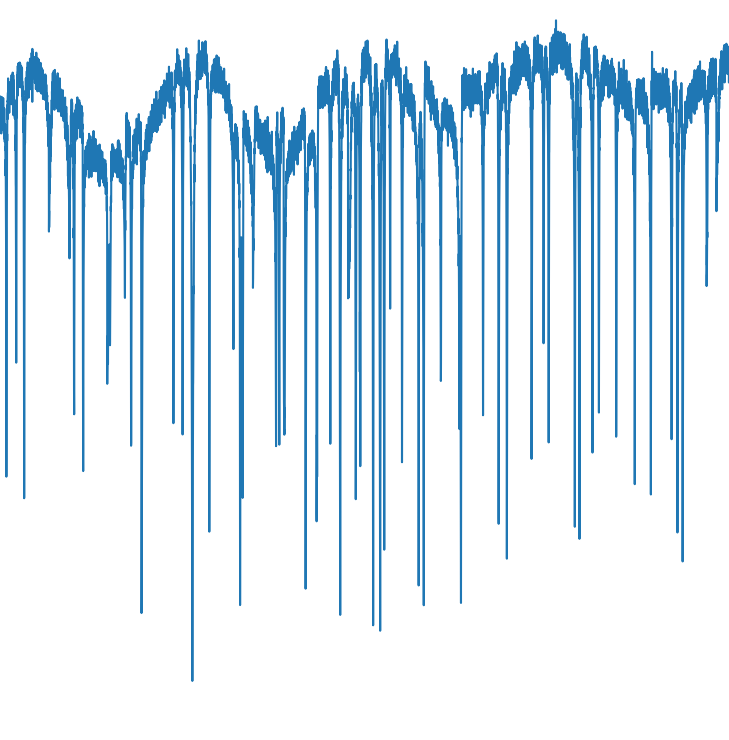
\includegraphics[width=.1\textwidth]{images/kid_example.png}};

    %\draw (5.5,-3) -- ++(0,-1);

    \draw [dash dot, rounded corners, fill=orange, fill opacity=0.12] (-2.5, 3.5) -- ++(0, -8) -- ++(-4,0) -- ++(0,8) -- ++(4,0)
    ; 
    \node () at (-4.5,2.75) {U-BOARD};

    \draw (1,0) -- ++(0,1.5) to [short, -o] (-2.45,1.5);
    \node () at (-1.5,1.75) {slow ADC};



\end{circuitikz}
    \caption{Caption}
    \label{fig:my_label}
\end{figure}



\end{document}